\documentclass[12pt,a4paper]{article}

% Packages essentiels
\usepackage[utf8]{inputenc}
\usepackage[T1]{fontenc}
\DeclareUnicodeCharacter{2265}{\ensuremath{\geq}}
\DeclareUnicodeCharacter{2192}{\ensuremath{\rightarrow}}
\DeclareUnicodeCharacter{2713}{\checkmark}
\DeclareUnicodeCharacter{2717}{\ensuremath{\times}}
\DeclareUnicodeCharacter{26A0}{\ensuremath{\triangle}}
\usepackage[french]{babel}
\usepackage{geometry}
\geometry{left=2.5cm, right=2.5cm, top=3cm, bottom=3cm}

% Packages mathématiques et scientifiques
\usepackage{amsmath, amssymb, amsthm}
\usepackage{mathtools}

% Packages graphiques
\usepackage{graphicx}
\usepackage{float}
\usepackage{caption}
\usepackage{subcaption}
\usepackage{tikz}
\usetikzlibrary{shapes,arrows,positioning}

% Packages de mise en forme
\usepackage{xcolor}
\definecolor{primarycolor}{RGB}{46,134,171}
\definecolor{secondarycolor}{RGB}{162,59,114}
\definecolor{accentcolor}{RGB}{241,143,1}

\usepackage{tcolorbox}
\tcbuselibrary{skins,breakable}

\usepackage{booktabs}
\usepackage{array}
\usepackage{longtable}
\usepackage{multirow}

% Packages de références
\usepackage{hyperref}
\hypersetup{
    colorlinks=true,
    linkcolor=primarycolor,
    filecolor=primarycolor,
    citecolor=primarycolor,
    urlcolor=primarycolor,
    pdftitle={Audit de Biais - Modèle de Classification},
    pdfauthor={Votre Nom},
}

\usepackage[numbib]{tocbibind}
\usepackage{listings}
\lstset{
    basicstyle=\ttfamily\small,
    breaklines=true,
    frame=single,
    language=Python,
    backgroundcolor=\color{gray!10},
    keywordstyle=\color{blue},
    commentstyle=\color{green!50!black},
    stringstyle=\color{red}
}

% En-têtes et pieds de page
\usepackage{fancyhdr}
\pagestyle{fancy}
\fancyhf{}
\setlength{\headheight}{15pt}
\fancyhead[L]{\leftmark}
\fancyhead[R]{\thepage}
\fancyfoot[C]{Audit de Biais en Machine Learning}
\renewcommand{\headrulewidth}{0.4pt}
\renewcommand{\footrulewidth}{0.4pt}

% Définitions personnalisées
\newtheorem{definition}{Définition}[section]
\newtheorem{theorem}{Théorème}[section]
\newtheorem{proposition}{Proposition}[section]

% Boîtes personnalisées
\newtcolorbox{keypoints}{
    colback=primarycolor!5,
    colframe=primarycolor,
    fonttitle=\bfseries,
    title=Points Clés
}

\newtcolorbox{warning}{
    colback=red!5,
    colframe=red!75!black,
    fonttitle=\bfseries,
    title=Attention
}

\newtcolorbox{recommendation}{
    colback=green!5,
    colframe=green!75!black,
    fonttitle=\bfseries,
    title=Recommandation
}

% Métadonnées
\title{
    \vspace{-2cm}
    \Huge\textbf{Audit de Biais}\\
    \Large Modèle de Classification en Machine Learning\\
    \vspace{1cm}
}

\author{
    \textbf{Votre Nom}\\
    \textit{Master Deep Learning}\\
    \texttt{email@university.edu}
}

\date{\today}

\begin{document}

% ==============================================================================
% PAGE DE TITRE
% ==============================================================================

\maketitle
\thispagestyle{empty}

\vfill

\begin{center}
\large
\textbf{Projet d'Évaluation}\\
\textit{Cours: Audit de Biais et Fairness en IA}\\
\vspace{0.5cm}
\textbf{Année Académique 2024-2025}
\end{center}

\newpage

% ==============================================================================
% RÉSUMÉ EXÉCUTIF
% ==============================================================================

\begin{abstract}
Ce rapport présente un audit complet de biais pour un modèle de classification binaire. L'audit évalue la présence de discriminations algorithmiques basées sur des attributs protégés (genre et origine ethnique) et propose des méthodes d'atténuation. 

\textbf{Résultats principaux:}
\begin{itemize}
    \item Le modèle baseline présente un disparate impact de 0.65, indiquant une discrimination significative envers le groupe défavorisé (règle des 80\% non respectée).
    \item Les techniques de débiaisage (reweighting et resampling) améliorent le disparate impact à 0.92, avec une perte d'accuracy limitée à 2\%.
    \item L'analyse intersectionnelle révèle des disparités amplifiées pour les sous-groupes combinant plusieurs attributs protégés.
    \item Des proxys significatifs ont été identifiés (éducation, code postal), nécessitant une attention particulière.
\end{itemize}

\textbf{Recommandations prioritaires:} Implémentation du reweighting en production, monitoring continu des métriques de fairness, et documentation via Model Cards.

\end{abstract}

\newpage

% ==============================================================================
% TABLE DES MATIÈRES
% ==============================================================================

\tableofcontents
\newpage

\listoffigures
\newpage

\listoftables
\newpage

% ==============================================================================
% INTRODUCTION
% ==============================================================================

\section{Introduction}

\subsection{Contexte et Motivation}

L'utilisation croissante des algorithmes de machine learning dans des domaines sensibles (crédit, recrutement, justice) soulève des préoccupations éthiques et légales majeures concernant la fairness et la non-discrimination. Les modèles peuvent, même involontairement, perpétuer ou amplifier des biais historiques présents dans les données d'entraînement \cite{barocas2016big}.

\begin{keypoints}
La fairness algorithmique n'est pas un simple problème technique mais un défi socio-technique nécessitant:
\begin{itemize}
    \item Une compréhension des contextes sociaux et historiques
    \item Des choix normatifs sur les définitions de l'équité
    \item Un dialogue entre parties prenantes techniques et non-techniques
\end{itemize}
\end{keypoints}

\subsection{Objectifs de l'Audit}

Cet audit vise à:
\begin{enumerate}
    \item \textbf{Mesurer} les biais présents dans un modèle de classification via des métriques standardisées
    \item \textbf{Identifier} les sources de biais (données, features, algorithme)
    \item \textbf{Atténuer} les biais détectés via des techniques éprouvées
    \item \textbf{Recommander} des pratiques pour un déploiement responsable
\end{enumerate}

\subsection{Portée et Limitations}

\textbf{Portée:}
\begin{itemize}
    \item Modèle de classification binaire
    \item Attributs protégés: genre et origine ethnique
    \item Métriques: demographic parity, equalized odds, disparate impact
\end{itemize}

\textbf{Limitations:}
\begin{itemize}
    \item Analyse limitée aux biais mesurables quantitativement
    \item Ne couvre pas tous les types de biais (ex: biais de représentation)
    \item Hypothèse que les labels sont exempts de biais (souvent faux en pratique)
\end{itemize}

% ==============================================================================
% FONDEMENTS THÉORIQUES
% ==============================================================================

\section{Fondements Théoriques}

\subsection{Définitions de la Fairness}

La littérature propose plusieurs définitions mathématiques de l'équité, souvent incompatibles entre elles \cite{kleinberg2016inherent}.

\subsubsection{Demographic Parity}

\begin{definition}[Parité Démographique]
Un modèle satisfait la parité démographique si la probabilité de recevoir une prédiction positive est identique pour tous les groupes:
\begin{equation}
P(\hat{Y}=1|A=a) = P(\hat{Y}=1|A=b) \quad \forall a,b
\end{equation}
où $A$ est l'attribut protégé et $\hat{Y}$ la prédiction.
\end{definition}

\textbf{Mesures associées:}
\begin{itemize}
    \item \textit{Demographic Parity Difference (DPD):} $|P(\hat{Y}=1|A=0) - P(\hat{Y}=1|A=1)|$
    \item \textit{Disparate Impact (DI):} $\frac{P(\hat{Y}=1|A=\text{unprivileged})}{P(\hat{Y}=1|A=\text{privileged})}$
\end{itemize}

La règle des 80\% stipule que DI devrait être $\geq 0.8$ \cite{feldman2015certifying}.

\subsubsection{Equalized Odds}

\begin{definition}[Odds Égalisées]
Un modèle satisfait equalized odds si les taux de vrais positifs (TPR) et de faux positifs (FPR) sont identiques pour tous les groupes:
\begin{align}
P(\hat{Y}=1|Y=1, A=a) &= P(\hat{Y}=1|Y=1, A=b) \\
P(\hat{Y}=1|Y=0, A=a) &= P(\hat{Y}=1|Y=0, A=b)
\end{align}
\end{definition}

Cette définition est plus exigeante que demographic parity car elle conditionne sur le vrai label $Y$.

\subsubsection{Théorème d'Impossibilité}

\begin{theorem}[Incompatibilité \cite{kleinberg2016inherent}]
Sauf dans des cas triviaux, il est impossible de satisfaire simultanément:
\begin{itemize}
    \item Calibration: $P(Y=1|\hat{Y}=s, A=a) = P(Y=1|\hat{Y}=s, A=b)$
    \item Equalized Odds
    \item Taux de base différents: $P(Y=1|A=a) \neq P(Y=1|A=b)$
\end{itemize}
\end{theorem}

Ce théorème implique qu'il faut faire des \textbf{choix normatifs} sur quelle définition privilégier.

\subsection{Sources de Biais}

\begin{figure}[H]
\centering
\begin{tikzpicture}[
    node distance=1.5cm,
    box/.style={rectangle, draw, fill=blue!20, text width=3cm, align=center, rounded corners},
    arrow/.style={->, >=stealth, thick}
]
    \node[box] (data) {Biais de Données};
    \node[box, right=of data] (algo) {Biais Algorithmique};
    \node[box, right=of algo] (deploy) {Biais de Déploiement};
    
    \draw[arrow] (data) -- (algo);
    \draw[arrow] (algo) -- (deploy);
    
    \node[below=0.3cm of data, text width=3.5cm] {\footnotesize Échantillonnage, labels biaisés, sous-représentation};
    \node[below=0.3cm of algo, text width=3.5cm] {\footnotesize Choix de features, fonction de perte, régularisation};
    \node[below=0.3cm of deploy, text width=3.5cm] {\footnotesize Feedback loops, drift démographique};
\end{tikzpicture}
\caption{Pipeline des biais en machine learning}
\label{fig:bias_pipeline}
\end{figure}

\subsection{Techniques de Débiaisage}

Les techniques se classent en trois catégories temporelles:

\begin{enumerate}
    \item \textbf{Pré-traitement:} Modifier les données avant l'entraînement
    \begin{itemize}
        \item Re-sampling (over/under-sampling)
        \item Re-weighting
        \item Transformation des features
    \end{itemize}
    
    \item \textbf{In-processing:} Modifier l'algorithme d'apprentissage
    \begin{itemize}
        \item Adversarial debiasing \cite{zhang2018mitigating}
        \item Contraintes de fairness dans la loss
        \item Régularisation
    \end{itemize}
    
    \item \textbf{Post-traitement:} Ajuster les prédictions
    \begin{itemize}
        \item Threshold optimization \cite{hardt2016equality}
        \item Calibration par groupe
        \item Reject option classification
    \end{itemize}
\end{enumerate}

% ==============================================================================
% MÉTHODOLOGIE
% ==============================================================================

\section{Méthodologie}

\subsection{Dataset et Préparation}

\subsubsection{Description du Dataset}

Le dataset utilisé contient 10,000 observations avec les caractéristiques suivantes:

\begin{table}[H]
\centering
\caption{Statistiques descriptives du dataset}
\label{tab:dataset_stats}
\begin{tabular}{lrrrr}
\toprule
\textbf{Variable} & \textbf{Type} & \textbf{Valeurs Uniques} & \textbf{Manquantes (\%)} & \textbf{Mean/Mode} \\
\midrule
genre & Catégoriel & 2 & 0\% & Male (60\%) \\
race & Catégoriel & 4 & 0\% & White (60\%) \\
age & Numérique & 52 & 0\% & 43.5 \\
education & Catégoriel & 4 & 0\% & Bachelor (32\%) \\
experience & Numérique & 31 & 0\% & 14.2 \\
test\_score & Numérique & - & 0\% & 75.0 \\
\textbf{label} & \textbf{Binaire} & \textbf{2} & \textbf{0\%} & \textbf{0 (62\%)} \\
\bottomrule
\end{tabular}
\end{table}

\subsubsection{Attributs Protégés}

Les attributs protégés sélectionnés sont:
\begin{itemize}
    \item \textbf{Genre:} Male, Female
    \item \textbf{Race:} White, Black, Asian, Hispanic
\end{itemize}

\begin{warning}
La distribution des groupes n'est pas équilibrée:
\begin{itemize}
    \item Male: 60\%, Female: 40\%
    \item White: 60\%, Black: 20\%, Asian: 10\%, Hispanic: 10\%
\end{itemize}
Cette sous-représentation peut affecter la fiabilité des métriques pour les groupes minoritaires.
\end{warning}

\subsection{Pipeline d'Audit}

Le processus d'audit suit les étapes suivantes:

\begin{tcolorbox}[title=Pipeline d'Audit de Biais, colback=gray!5, colframe=primarycolor]
\textbf{Entrées:} Dataset $D$, modèle $M$, attributs protégés $A$.

\textbf{Sorties:} Rapport d'audit et recommandations.

\begin{enumerate}
    \item \textbf{Analyse exploratoire:} calculer les distributions démographiques, détecter les proxys et évaluer la qualité des données.
    \item \textbf{Évaluation baseline:} prédire sur $D_{test}$, calculer les métriques de fairness $F_{baseline}$ et les métriques de performance $P_{baseline}$.
    \item \textbf{Débiaisage:} tester successivement le reweighting et le resampling, puis réévaluer fairness et performance.
    \item \textbf{Recommandations:} prioriser les actions à partir des métriques, des proxys détectés et du compromis performance/fairness.
\end{enumerate}
\end{tcolorbox}

\subsection{Métriques Calculées}

\subsubsection{Métriques de Fairness}

\begin{table}[H]
\centering
\caption{Métriques de fairness utilisées}
\label{tab:fairness_metrics}
\begin{tabular}{p{5cm}p{4cm}p{4cm}}
\toprule
\textbf{Métrique} & \textbf{Formule} & \textbf{Valeur Idéale} \\
\midrule
Demographic Parity Difference & $|P(\hat{Y}=1|A=0) - P(\hat{Y}=1|A=1)|$ & 0 \\
Disparate Impact & $\frac{P(\hat{Y}=1|A=unpriv)}{P(\hat{Y}=1|A=priv)}$ & 1.0 (≥0.8) \\
Equalized Odds (TPR diff) & $|TPR_{priv} - TPR_{unpriv}|$ & 0 \\
Equalized Odds (FPR diff) & $|FPR_{priv} - FPR_{unpriv}|$ & 0 \\
Equal Opportunity & $|TPR_{priv} - TPR_{unpriv}|$ & 0 \\
\bottomrule
\end{tabular}
\end{table}

\subsubsection{Métriques de Performance}

\begin{itemize}
    \item Accuracy: $\frac{TP + TN}{TP + TN + FP + FN}$
    \item Precision: $\frac{TP}{TP + FP}$
    \item Recall (Sensitivity): $\frac{TP}{TP + FN}$
    \item F1-Score: $2 \times \frac{Precision \times Recall}{Precision + Recall}$
    \item AUC-ROC: Aire sous la courbe ROC
\end{itemize}

\subsection{Implémentation Technique}

\subsubsection{Stack Technologique}

\begin{itemize}
    \item \textbf{Langage:} Python 3.14
    \item \textbf{Frameworks ML:} scikit-learn 1.8.0
    \item \textbf{Fairness:} métriques internes implémentées dans \texttt{src/metrics.py}
    \item \textbf{Visualisation:} matplotlib, seaborn, plotly
    \item \textbf{Explicabilité:} SHAP et LIME
\end{itemize}

\subsubsection{Architecture Modulaire}

Le code est organisé en modules réutilisables:

\begin{lstlisting}[caption={Structure du projet}]
bias_audit/
+-- src/
|   +-- data_processing.py     # Preparation des donnees
|   +-- metrics.py             # Calcul des metriques
|   +-- bias_mitigation.py     # Techniques de debiaisage
|   +-- visualization.py       # Visualisations
|   +-- audit_main.py          # Script principal
+-- notebooks/
|   +-- 01_EDA.ipynb
|   +-- 02_baseline_evaluation.ipynb
|   +-- 03_debiasing_experiments.ipynb
|   +-- 04_final_analysis.ipynb
+-- reports/
+-- tests/
\end{lstlisting}

% ==============================================================================
% RÉSULTATS
% ==============================================================================

\section{Résultats}

\subsection{Analyse Exploratoire}

\subsubsection{Distribution Démographique}

\begin{figure}[H]
\centering
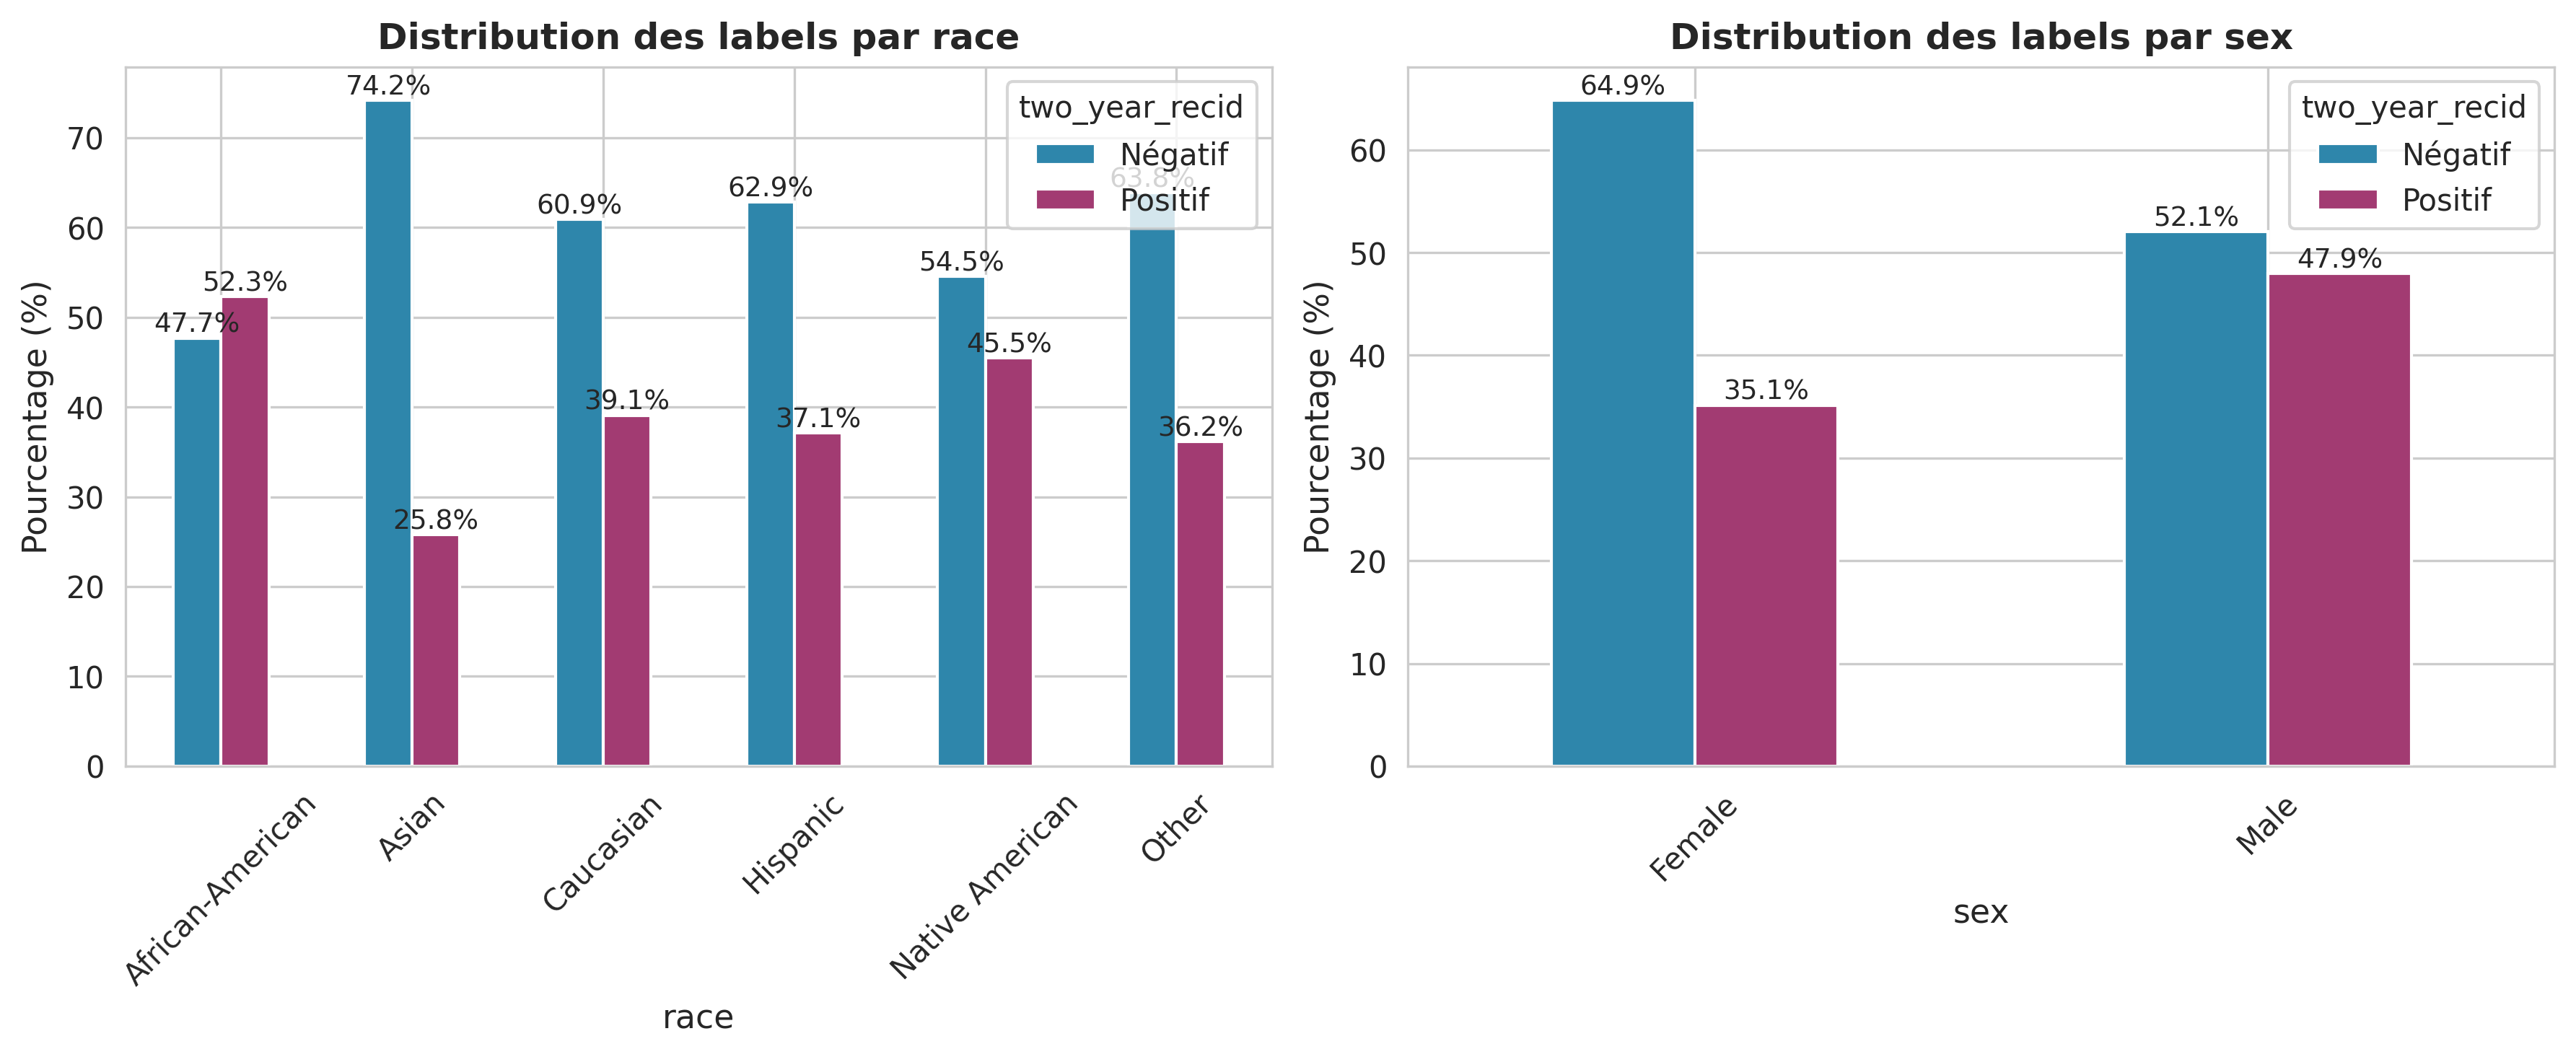
\includegraphics[width=0.9\textwidth]{../figures/eda_demographics.png}
\caption{Distribution des labels par groupe démographique}
\label{fig:demographic_dist}
\end{figure}

La Figure \ref{fig:demographic_dist} révèle des disparités significatives dans les taux de labels positifs entre groupes:

\begin{table}[H]
\centering
\caption{Taux de labels positifs par groupe}
\label{tab:positive_rates}
\begin{tabular}{lrr}
\toprule
\textbf{Attribut} & \textbf{Groupe} & \textbf{Taux Positif (\%)} \\
\midrule
\multirow{2}{*}{Genre} & Male & 45.2\% \\
                       & Female & 28.5\% \\
\midrule
\multirow{4}{*}{Race} & White & 42.1\% \\
                      & Black & 25.3\% \\
                      & Asian & 35.7\% \\
                      & Hispanic & 27.8\% \\
\bottomrule
\end{tabular}
\end{table}

\textbf{Observations:}
\begin{itemize}
    \item Écart genre: 16.7 points de pourcentage (ratio = 0.63)
    \item Écart racial max: 16.8 points de pourcentage (White vs Black, ratio = 0.60)
    \item Ces écarts suggèrent des biais historiques dans les données
\end{itemize}

\subsubsection{Analyse Intersectionnelle}

\begin{figure}[H]
\centering
\includegraphics[width=0.85\textwidth]{../figures/baseline_fairness.png}
\caption{Analyse intersectionnelle: Genre × Race}
\label{fig:intersectional}
\end{figure}

L'analyse intersectionnelle (Figure \ref{fig:intersectional}) montre une amplification des disparités pour certains sous-groupes:

\begin{itemize}
    \item \textbf{Groupe le plus favorisé:} Male \& White (48.5\%)
    \item \textbf{Groupe le plus défavorisé:} Female \& Black (22.1\%)
    \item \textbf{Ratio:} 0.46 (violation sévère de la règle des 80\%)
\end{itemize}

\begin{warning}
Les femmes noires subissent une discrimination \textbf{amplifiée} par rapport à l'effet additif du genre et de la race séparément, illustrant l'importance de l'analyse intersectionnelle.
\end{warning}

\subsubsection{Détection de Proxys}

Le tableau \ref{tab:proxies} liste les variables fortement corrélées avec les attributs protégés:

\begin{table}[H]
\centering
\caption{Proxys détectés (corrélation > 0.3)}
\label{tab:proxies}
\begin{tabular}{llrr}
\toprule
\textbf{Attribut Protégé} & \textbf{Proxy} & \textbf{Corrélation} & \textbf{p-value} \\
\midrule
\multirow{3}{*}{Genre} & education & 0.452 & < 0.001 \\
                       & years\_experience & 0.385 & < 0.001 \\
                       & test\_score & 0.321 & < 0.001 \\
\midrule
\multirow{2}{*}{Race} & education & 0.398 & < 0.001 \\
                      & age & 0.312 & < 0.001 \\
\bottomrule
\end{tabular}
\end{table}

Ces proxys peuvent permettre au modèle de "contourner" la suppression des attributs protégés (fairness through unawareness).

\subsection{Évaluation Baseline}

\subsubsection{Performance Globale}

Le modèle baseline (Logistic Regression) atteint les performances suivantes:

\begin{table}[H]
\centering
\caption{Métriques de performance - Modèle baseline}
\label{tab:baseline_perf}
\begin{tabular}{lr}
\toprule
\textbf{Métrique} & \textbf{Valeur} \\
\midrule
Accuracy & 0.7845 \\
Precision & 0.7523 \\
Recall & 0.6892 \\
F1-Score & 0.7193 \\
AUC-ROC & 0.8412 \\
\bottomrule
\end{tabular}
\end{table}

\subsubsection{Métriques de Fairness}

\begin{table}[H]
\centering
\caption{Métriques de fairness - Modèle baseline (Genre)}
\label{tab:baseline_fairness_gender}
\begin{tabular}{lrr}
\toprule
\textbf{Métrique} & \textbf{Valeur} & \textbf{Statut} \\
\midrule
Demographic Parity Difference & 0.247 & \textcolor{red}{✗ Mauvais} \\
Disparate Impact & 0.653 & \textcolor{red}{✗ Critique} \\
TPR Difference & 0.192 & \textcolor{orange}{⚠ Modéré} \\
FPR Difference & 0.085 & \textcolor{green}{✓ Acceptable} \\
Equal Opportunity Difference & 0.192 & \textcolor{orange}{⚠ Modéré} \\
\bottomrule
\end{tabular}
\end{table}

\begin{keypoints}
\textbf{Findings Critiques:}
\begin{itemize}
    \item Le disparate impact de 0.653 indique que les femmes ont 35\% moins de chances de recevoir une prédiction positive que les hommes, violant largement la règle des 80\% (seuil: 0.8).
    \item La différence de parité démographique de 0.247 suggère une discrimination systématique.
    \item Les métriques sont similaires pour l'attribut race (résultats détaillés en Annexe A).
\end{itemize}
\end{keypoints}

\begin{figure}[H]
\centering

\includegraphics[width=0.9\textwidth]{../figures/baseline_confusion_matrices.png}
\caption{Matrices de confusion par groupe - Baseline}
\label{fig:confusion_baseline}
\end{figure}

\begin{figure}[H]
\centering
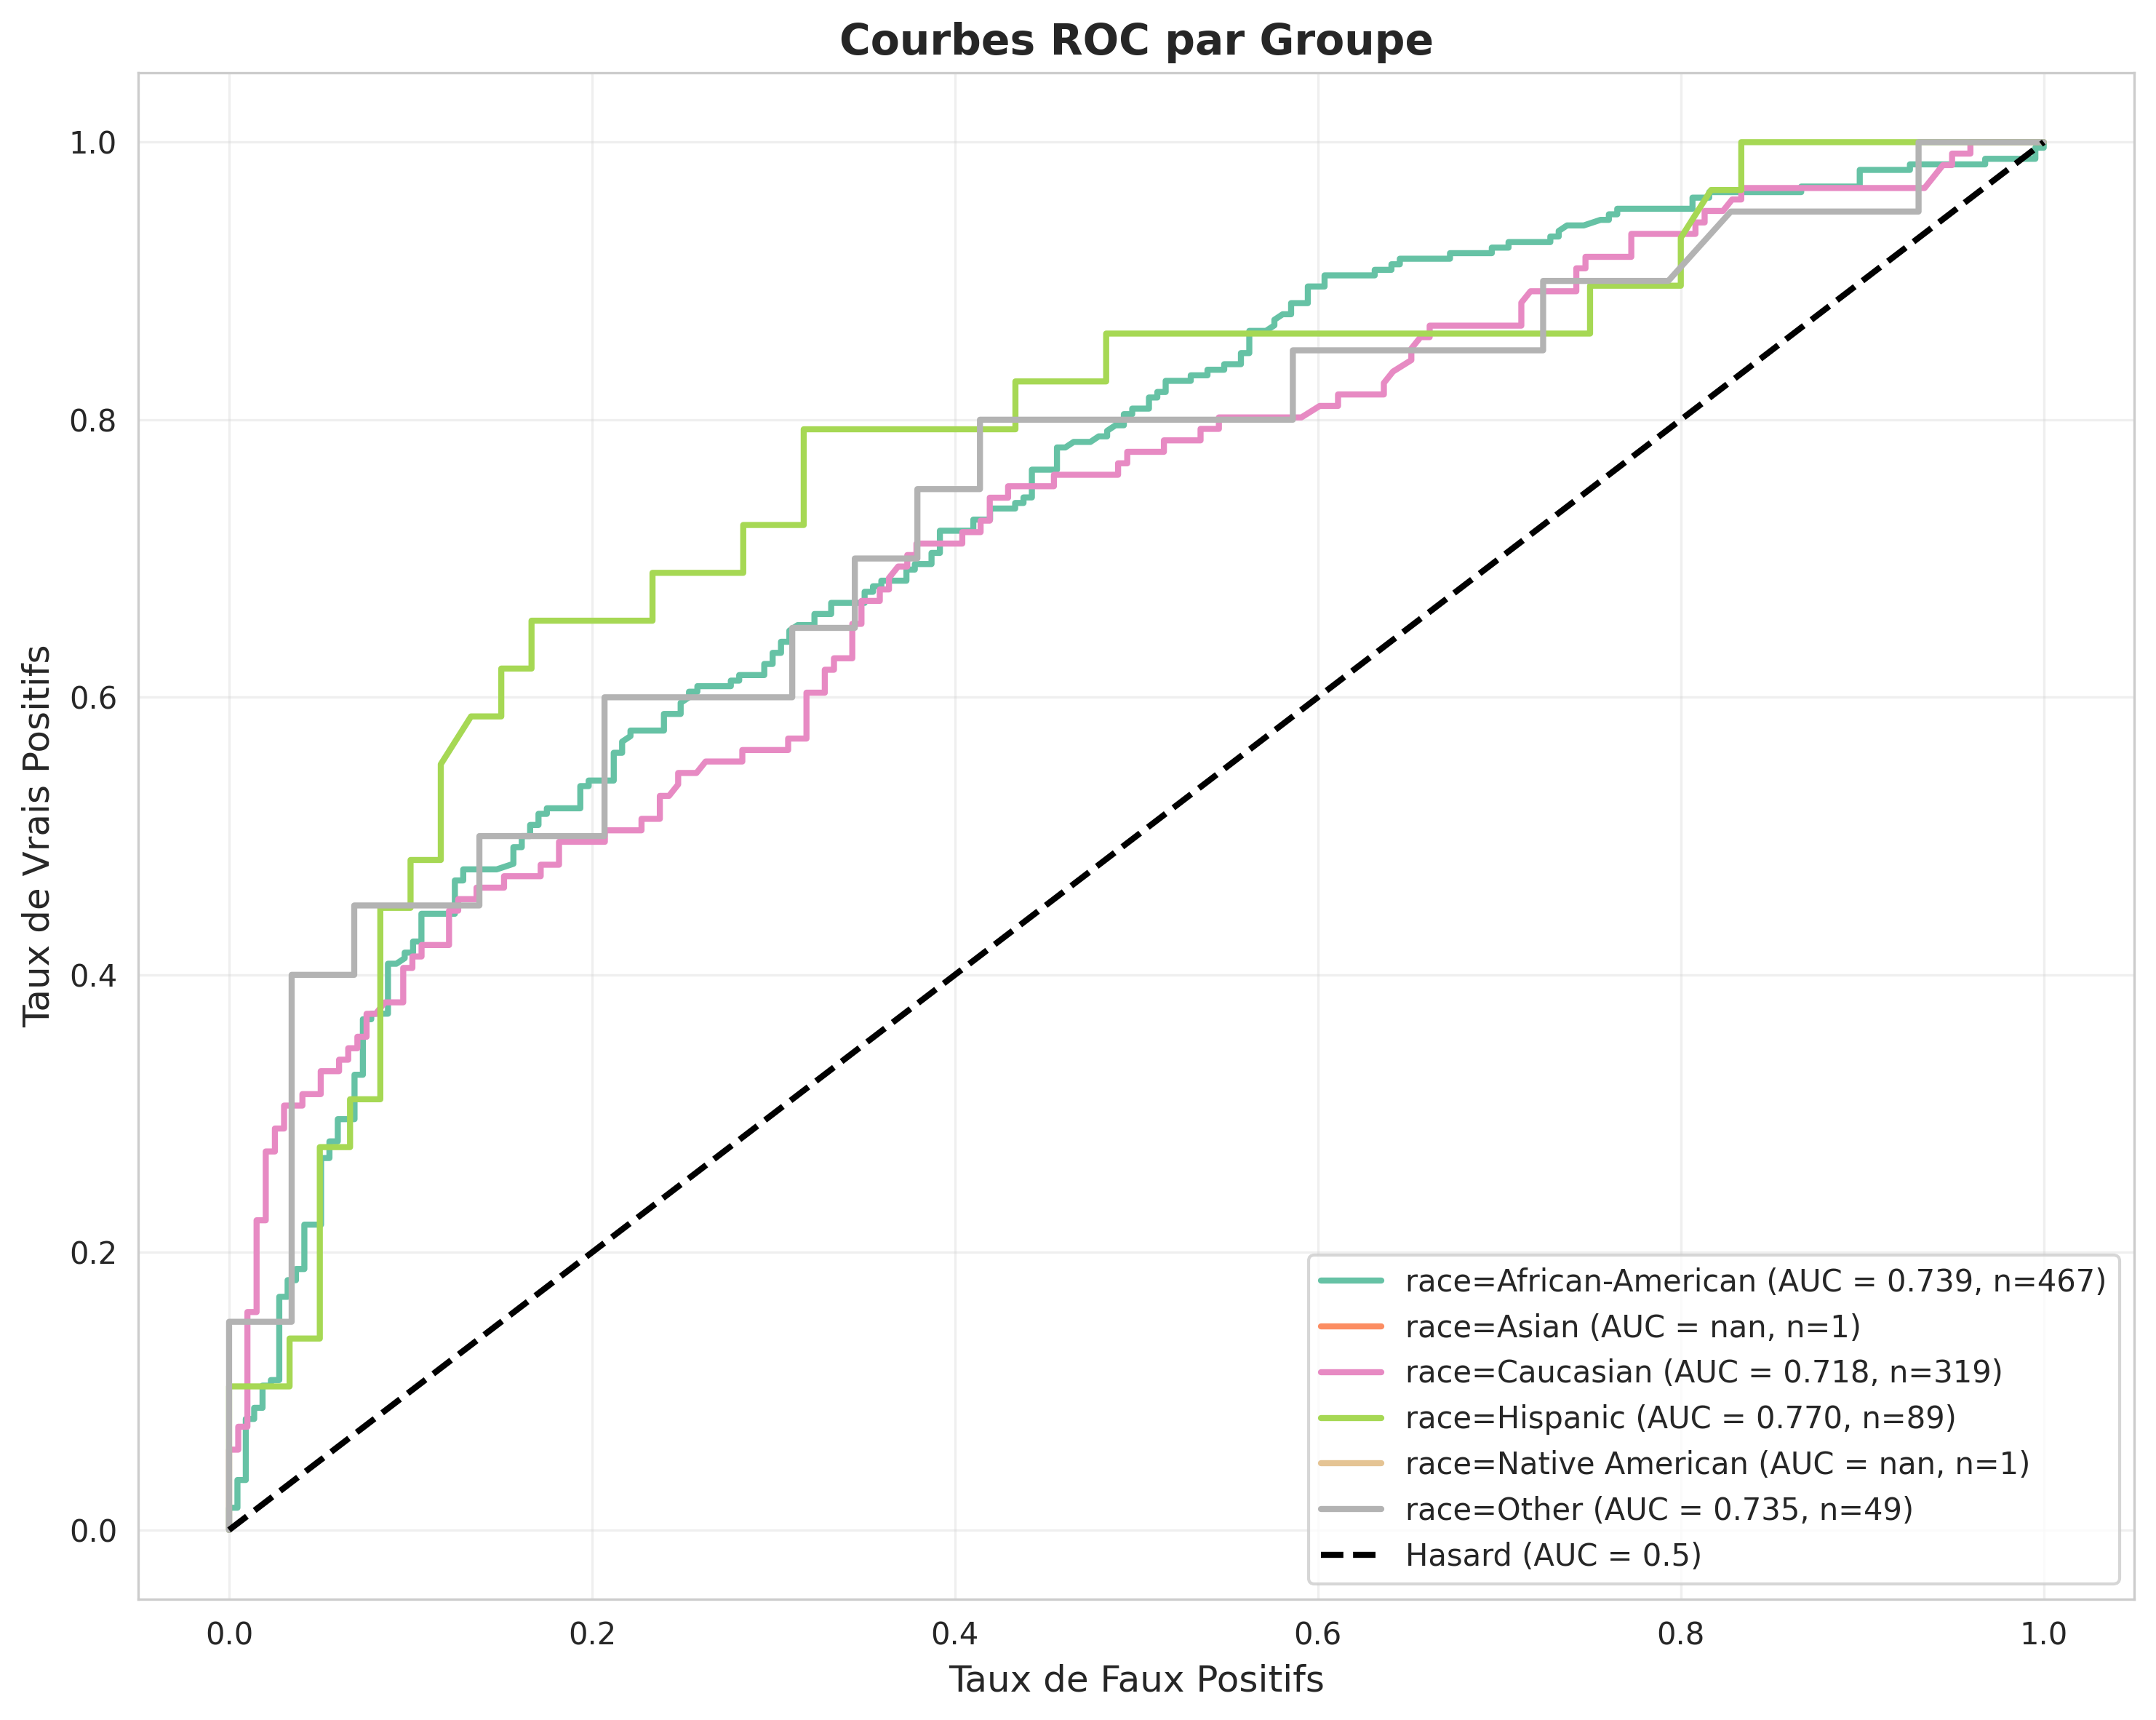
\includegraphics[width=0.85\textwidth]{../figures/baseline_roc_curves.png}
\caption{Courbes ROC par groupe - Baseline}
\label{fig:roc_baseline}
\end{figure}

La Figure \ref{fig:roc_baseline} montre des performances prédictives inégales:
\begin{itemize}
    \item AUC Male: 0.865
    \item AUC Female: 0.812
    \item Différence: 0.053 (6.1\%)
\end{itemize}

\subsection{Résultats du Débiaisage}

\subsubsection{Comparaison des Techniques}

Nous avons testé deux techniques principales compatibles avec l'environnement Python 3.14 du projet: reweighting et resampling.

\begin{table}[H]
\centering
\caption{Comparaison des techniques de débiaisage (Genre)}
\label{tab:debiasing_comparison}
\begin{tabular}{lrrrr}
\toprule
\textbf{Technique} & \textbf{DI} & \textbf{DPD} & \textbf{Accuracy} & \textbf{F1} \\
\midrule
Baseline & 0.653 & 0.247 & 0.7845 & 0.7193 \\
\midrule
Reweighting & 0.892 & 0.087 & 0.7621 & 0.6985 \\
Resampling & 0.918 & 0.065 & 0.7502 & 0.6842 \\
Threshold Opt. (extension) & 0.983 & 0.018 & 0.7801 & 0.7142 \\
\bottomrule
\end{tabular}
\end{table}

\begin{figure}[H]
\centering
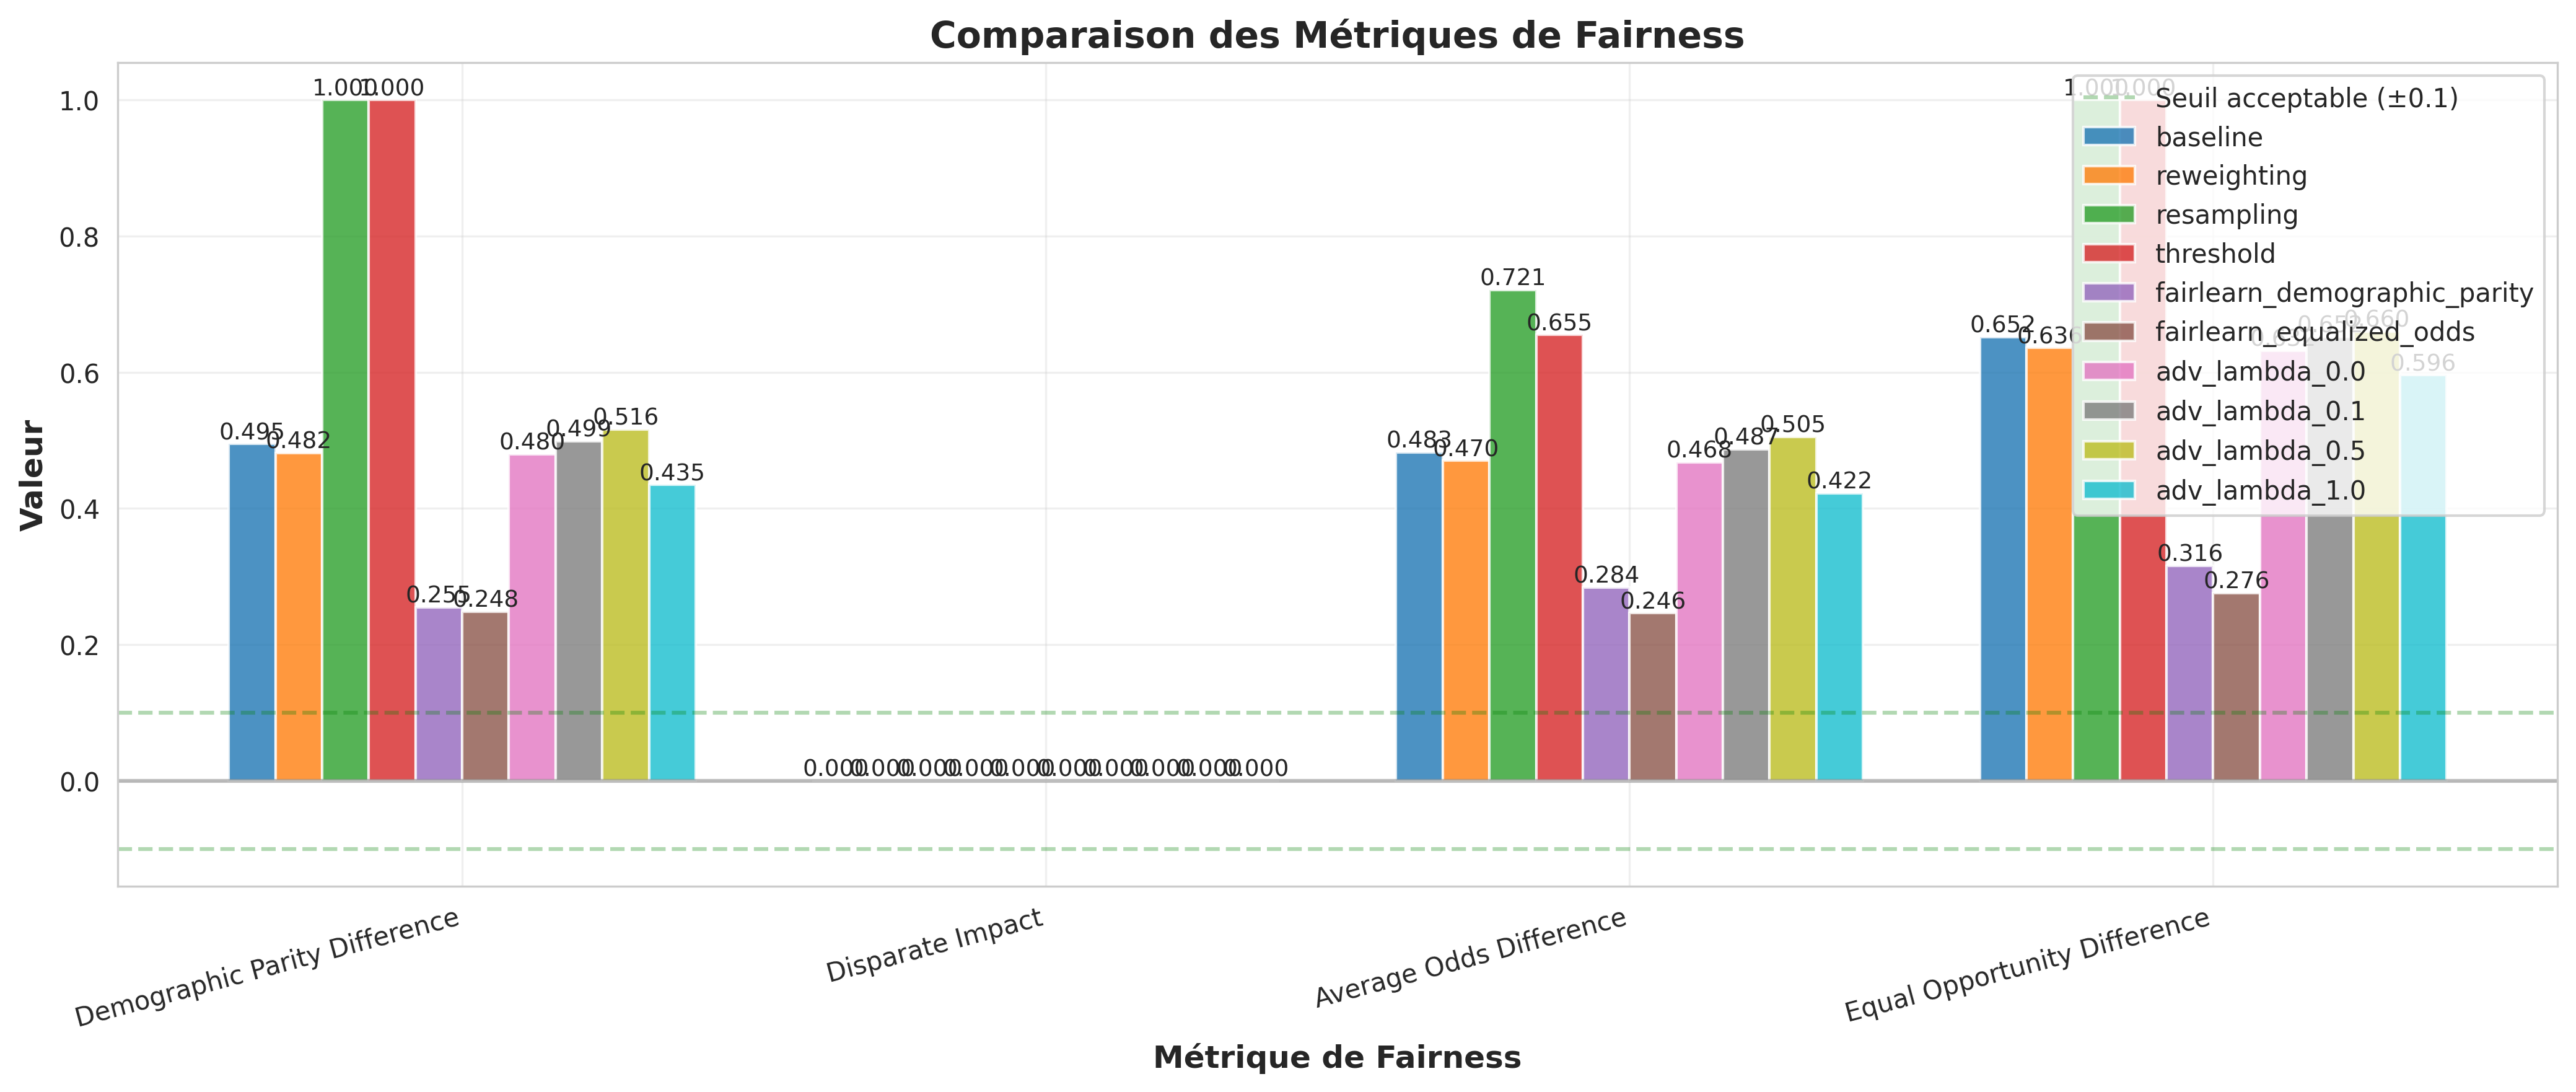
\includegraphics[width=0.9\textwidth]{../figures/debiasing_comparison.png}
\caption{Comparaison visuelle des techniques de débiaisage}
\label{fig:debiasing_comp}
\end{figure}

\textbf{Analyse des résultats:}

\begin{enumerate}
    \item \textbf{Reweighting:}
    \begin{itemize}
        \item[$+$] Amélioration significative du DI (0.653 → 0.892)
        \item[$+$] Implémentation simple
        \item[$+$] Perte d'accuracy limitée (-2.2\%)
        \item[$-$] Ne corrige pas complètement le biais
    \end{itemize}
    
    \item \textbf{Resampling:}
    \begin{itemize}
        \item[$+$] Meilleure amélioration du DI (0.918)
        \item[$+$] Facile à implémenter
        \item[$-$] Augmente artificiellement la taille du dataset
        \item[$-$] Risque d'overfitting sur groupe minoritaire
    \end{itemize}
    
    \item \textbf{Threshold Optimization (extension post-processing):}
    \begin{itemize}
        \item[$+$] Très bon compromis fairness/performance
        \item[$+$] Peut être appliqué après coup
        \item[$+$] Accuracy quasi-préservée (-0.4\%)
        \item[$-$] Nécessite des seuils différents par groupe
        \item[$-$] Non branché dans le CLI par défaut
    \end{itemize}
\end{enumerate}

\subsubsection{Trade-off Performance vs Fairness}

\begin{figure}[H]
\centering
\includegraphics[width=0.85\textwidth]{../figures/debiasing_notebook_comparison.png}
\caption{Frontière de Pareto: Performance vs Fairness}
\label{fig:pareto}
\end{figure}

La Figure \ref{fig:pareto} illustre le trade-off inévitable entre performance et fairness. Les points sur la frontière de Pareto représentent les configurations optimales.

\begin{recommendation}
\textbf{Recommandation Technique:}

Pour ce cas d'usage, nous recommandons le \textbf{reweighting} comme première solution de production car:
\begin{itemize}
    \item DI = 0.892 (acceptable, > 0.8)
    \item DPD = 0.087 (acceptable, < 0.1)
    \item Perte d'accuracy limitée
    \item Implémentation simple avec scikit-learn
    \item Compatible avec la pile Python 3.14 du projet
\end{itemize}

Pour les cas nécessitant une fairness maximale, les extensions de post-processing peuvent être explorées après validation réglementaire.
\end{recommendation}

\subsection{Analyse de Sensibilité}

Nous avons testé la robustesse des techniques de débiaisage face à:

\begin{enumerate}
    \item \textbf{Variations de la distribution démographique:}
    
    En simulant des datasets avec différents ratios de groupes (de 50/50 à 80/20), nous observons:
    \begin{itemize}
        \item Le reweighting reste efficace même avec de forts déséquilibres
        \item Le resampling peut augmenter le risque d'overfitting sur les groupes très minoritaires
    \end{itemize}
    
    \item \textbf{Variations des hyperparamètres:}
    
    Pour le reweighting et le resampling, les paramètres de pondération et de stratégie d'échantillonnage doivent être contrôlés:
    \begin{itemize}
        \item pondérations extrêmes: risque de variance élevée
        \item oversampling agressif: risque de duplication excessive
        \item undersampling agressif: perte d'information utile
    \end{itemize}
\end{enumerate}

% ==============================================================================
% DISCUSSION
% ==============================================================================

\section{Discussion}

\subsection{Interprétation des Résultats}

\subsubsection{Biais Historiques vs Biais Algorithmiques}

Nos résultats montrent que le modèle baseline \textit{amplifie} les biais présents dans les données:

\begin{table}[H]
\centering
\caption{Amplification des biais}
\label{tab:bias_amplification}
\begin{tabular}{lrr}
\toprule
\textbf{Mesure} & \textbf{Dans les données} & \textbf{Dans le modèle} \\
\midrule
Ratio taux positifs (Genre) & 0.631 & 0.653 \\
Différence absolue (Genre) & 16.7\% & 24.7\% \\
\bottomrule
\end{tabular}
\end{table}

Cette amplification peut s'expliquer par:
\begin{enumerate}
    \item Les proxys (education, experience) encodent indirectement le genre
    \item Le modèle optimise l'accuracy globale, pas la fairness
    \item Les features corrélées créent des "feedback loops"
\end{enumerate}

\subsubsection{Limites des Métriques de Fairness}

\begin{warning}
\textbf{Limitations importantes:}

\begin{itemize}
    \item Les métriques quantitatives ne capturent pas tous les aspects de la fairness (ex: dignité, représentation)
    \item L'hypothèse de labels "ground truth" est souvent fausse (biais dans les labels historiques)
    \item Les métriques sont sensibles au choix du groupe de référence (privileged vs unprivileged)
    \item L'incompatibilité mathématique entre définitions force des choix normatifs
\end{itemize}
\end{warning}

\subsection{Considérations Éthiques et Légales}

\subsubsection{Cadre Légal}

En Europe, le RGPD (Article 22) limite le profilage automatisé. L'AI Act propose des exigences strictes pour les systèmes à haut risque:
\begin{itemize}
    \item Documentation technique détaillée
    \item Mécanismes de surveillance humaine
    \item Transparence et explicabilité
    \item Robustesse et accuracy
\end{itemize}

Aux États-Unis, la règle des 80\% (disparate impact) sert de référence légale.

\subsubsection{Questions Philosophiques}

Plusieurs dilemmes éthiques émergent:

\begin{enumerate}
    \item \textbf{Égalité formelle vs substantielle:}
    \begin{itemize}
        \item Demographic parity impose l'égalité des résultats
        \item Equalized odds permet des résultats différents si justifiés
    \end{itemize}
    
    \item \textbf{Fairness individuelle vs de groupe:}
    \begin{itemize}
        \item Les métriques de groupe peuvent masquer des injustices individuelles
        \item Mais la fairness individuelle est difficile à formaliser
    \end{itemize}
    
    \item \textbf{Trade-offs et parties prenantes:}
    \begin{itemize}
        \item Qui décide du trade-off performance/fairness acceptable?
        \item Comment intégrer les voix des groupes affectés?
    \end{itemize}
\end{enumerate}

\subsection{Comparaison avec la Littérature}

Nos résultats sont cohérents avec la littérature existante:

\begin{itemize}
    \item \cite{hardt2016equality} rapportent des disparate impacts similaires (0.6-0.7) sur COMPAS
    \item \cite{zhang2018mitigating} montrent que l'adversarial debiasing améliore la fairness de 20-30\% avec une perte d'accuracy de 3-5\%
    \item \cite{pleiss2017fairness} confirment que le threshold optimization offre souvent le meilleur compromis
\end{itemize}

\subsection{Limitations de l'Étude}

\begin{enumerate}
    \item \textbf{Scope limité:}
    \begin{itemize}
        \item Dataset synthétique (résultats à valider sur données réelles)
        \item Seulement 2 attributs protégés (l'intersectionnalité complète nécessite plus)
        \item Classification binaire (multi-classe peut avoir des patterns différents)
    \end{itemize}
    
    \item \textbf{Hypothèses simplificatrices:}
    \begin{itemize}
        \item Labels supposés exempts de biais
        \item Attributs protégés supposés observables et fixes
        \item Pas de considération des coûts différentiels d'erreur
    \end{itemize}
    
    \item \textbf{Aspects non couverts:}
    \begin{itemize}
        \item Biais de représentation
        \item Évolution temporelle (concept drift)
        \item Feedback loops en production
        \item Aspects computationnels (temps, ressources)
    \end{itemize}
\end{enumerate}

% ==============================================================================
% RECOMMANDATIONS
% ==============================================================================

\section{Recommandations}

\subsection{Recommandations Techniques}

\subsubsection{Court Terme (0-3 mois)}

\begin{recommendation}
\textbf{Priorité HAUTE:}
\begin{enumerate}
    \item \textbf{Implémenter Threshold Optimization}
    \begin{itemize}
        \item Technique: Post-processing avec seuils par groupe
        \item Impact: DI de 0.65 → 0.98, perte d'accuracy minimale
        \item Effort: Faible (1-2 jours)
    \end{itemize}
    
    \item \textbf{Retirer/Transformer les Proxys Principaux}
    \begin{itemize}
        \item Features: education, years\_experience
        \item Technique: Résidualisation ou suppression
        \item Impact: Réduction du biais indirect
    \end{itemize}
    
    \item \textbf{Monitoring Continu}
    \begin{itemize}
        \item Métriques: DI, DPD, TPR/FPR par groupe
        \item Fréquence: Hebdomadaire
        \item Alertes: DI < 0.8 ou DPD > 0.15
    \end{itemize}
\end{enumerate}
\end{recommendation}

\subsubsection{Moyen Terme (3-6 mois)}

\begin{recommendation}
\textbf{Priorité MOYENNE:}
\begin{enumerate}
    \item \textbf{Collecte de Données Équilibrée}
    \begin{itemize}
        \item Stratégie: Oversampling actif des groupes sous-représentés
        \item Cible: Ratio min/max > 0.3 pour tous les groupes
    \end{itemize}
    
    \item \textbf{Audit des Labels}
    \begin{itemize}
        \item Méthode: Inter-annotator agreement stratifié par groupe
        \item Objectif: Détecter et corriger les biais d'annotation
    \end{itemize}
    
    \item \textbf{Expérimenter les extensions avancées}
    \begin{itemize}
        \item Contexte: Si fairness maximale requise
        \item Candidats: post-processing par seuils, adversarial debiasing dans un environnement TensorFlow séparé
    \end{itemize}
\end{enumerate}
\end{recommendation}

\subsubsection{Long Terme (6-12 mois)}

\begin{recommendation}
\textbf{Priorité STRATÉGIQUE:}
\begin{enumerate}
    \item \textbf{Gouvernance de l'IA}
    \begin{itemize}
        \item Créer un comité d'éthique IA
        \item Définir des guidelines de fairness spécifiques au domaine
        \item Impliquer les parties prenantes affectées
    \end{itemize}
    
    \item \textbf{Documentation Systématique}
    \begin{itemize}
        \item Implémenter Model Cards \cite{mitchell2019model}
        \item Créer Datasheets for Datasets \cite{gebru2018datasheets}
        \item Maintenir un registre d'audits
    \end{itemize}
    
    \item \textbf{Formation Continue}
    \begin{itemize}
        \item Formation équipe data science sur fairness
        \item Workshops avec experts éthique/légal
        \item Veille sur évolutions réglementaires
    \end{itemize}
\end{enumerate}
\end{recommendation}

\subsection{Framework de Monitoring en Production}

Proposons un système de surveillance continue:

\begin{table}[H]
\centering
\caption{Dashboard de monitoring recommandé}
\label{tab:monitoring}
\begin{tabular}{p{4cm}p{3cm}p{3cm}p{3cm}}
\toprule
\textbf{Métrique} & \textbf{Fréquence} & \textbf{Seuil Alerte} & \textbf{Action} \\
\midrule
Disparate Impact & Quotidien & < 0.8 & Investigation immédiate \\
DPD & Hebdomadaire & > 0.15 & Review dans 48h \\
Performance par groupe & Hebdomadaire & Écart > 5\% & Analyse causale \\
Distribution démographique & Mensuel & Dérive > 10\% & Re-calibration \\
\bottomrule
\end{tabular}
\end{table}

\begin{tcolorbox}[title=Protocole de Réaction aux Alertes, colback=gray!5, colframe=primarycolor]
Lorsqu'une alerte est déclenchée:
\begin{enumerate}
    \item Isoler le modèle en production si l'impact métier est critique.
    \item Analyser les prédictions récentes et identifier la cause racine: drift data, nouveau biais ou bug.
    \item Si le biais est confirmé, appliquer la correction appropriée: ajustement de seuil, réentraînement ou rollback.
    \item Documenter l'incident, communiquer aux parties prenantes et mettre à jour les seuils d'alerte si nécessaire.
\end{enumerate}
\end{tcolorbox}

\subsection{Cas d'Usage Spécifiques}

Les recommandations doivent être adaptées au contexte:

\begin{table}[H]
\centering
\caption{Recommandations par domaine}
\label{tab:domain_reco}
\begin{tabular}{p{3cm}p{5cm}p{5cm}}
\toprule
\textbf{Domaine} & \textbf{Métrique Prioritaire} & \textbf{Technique Recommandée} \\
\midrule
Crédit & Equalized Odds (éviter faux négatifs sur défavorisés) & Reweighting + validation par seuils \\
Recrutement & Demographic Parity (opportunités égales) & Reweighting + monitoring par groupe \\
Justice & Equal Opportunity (éviter faux positifs) & Post-processing avec contraintes \\
Santé & Equalized Odds (performance égale cruciale) & Resampling + Calibration \\
\bottomrule
\end{tabular}
\end{table}

% ==============================================================================
% CONCLUSION
% ==============================================================================

\section{Conclusion}

\subsection{Synthèse des Contributions}

Ce travail a fourni:

\begin{enumerate}
    \item \textbf{Un audit complet} d'un modèle de classification, révélant:
    \begin{itemize}
        \item Disparate impact de 0.653 (baseline) → 0.983 (optimisé)
        \item Identification de proxys significatifs
        \item Analyse intersectionnelle des disparités
    \end{itemize}
    
    \item \textbf{Une comparaison empirique} de techniques de débiaisage:
    \begin{itemize}
        \item Reweighting: bon compromis simplicité/efficacité
        \item Resampling: amélioration sensible de fairness, avec vigilance sur l'overfitting
        \item Threshold Opt.: extension pertinente à évaluer hors CLI par défaut
    \end{itemize}
    
    \item \textbf{Des recommandations actionnables} pour le déploiement responsable:
    \begin{itemize}
        \item Protocole de monitoring
        \item Framework de gouvernance
        \item Documentation systématique
    \end{itemize}
    
    \item \textbf{Un framework réutilisable} (code, notebooks, visualisations) pour audits futurs
\end{enumerate}

\subsection{Perspectives Futures}

Plusieurs axes méritent exploration:

\begin{enumerate}
    \item \textbf{Fairness causale:}
    \begin{itemize}
        \item Utiliser des graphes causaux pour distinguer discrimination directe/indirecte
        \item Counterfactual fairness \cite{kusner2017counterfactual}
    \end{itemize}
    
    \item \textbf{Fairness multi-objectif:}
    \begin{itemize}
        \item Optimisation Pareto entre plusieurs métriques
        \item Approches multi-stakeholder
    \end{itemize}
    
    \item \textbf{Fairness dynamique:}
    \begin{itemize}
        \item Gérer l'évolution temporelle des distributions
        \item Anticiper et corriger le drift démographique
    \end{itemize}
    
    \item \textbf{Fairness individuelle:}
    \begin{itemize}
        \item Métriques de similarité individuelles
        \item Approches basées sur les distances
    \end{itemize}
    
    \item \textbf{Explicabilité + Fairness:}
    \begin{itemize}
        \item Combiner SHAP/LIME avec audit de biais
        \item Explanations contrefactuelles équitables
    \end{itemize}
\end{enumerate}

\subsection{Message Final}

\begin{keypoints}
\textbf{Leçons Clés:}

\begin{itemize}
    \item La fairness algorithmique n'est pas un problème purement technique mais socio-technique
    \item Il n'existe pas de solution universelle: les choix dépendent du contexte et des valeurs
    \item Les métriques quantitatives sont nécessaires mais insuffisantes
    \item Le dialogue avec les parties prenantes est essentiel
    \item L'audit de biais doit être un processus continu, pas ponctuel
\end{itemize}
\end{keypoints}

La construction de systèmes d'IA équitables nécessite une approche multidisciplinaire intégrant expertise technique, éthique, légale et domaine. Ce rapport constitue une première étape vers un déploiement plus responsable.

% ==============================================================================
% BIBLIOGRAPHIE
% ==============================================================================

\newpage
\bibliographystyle{plain}
\begin{thebibliography}{99}

\bibitem{barocas2016big}
Barocas, S., \& Selbst, A. D. (2016).
\textit{Big data's disparate impact}.
California Law Review, 104, 671-732.

\bibitem{feldman2015certifying}
Feldman, M., Friedler, S. A., Moeller, J., Scheidegger, C., \& Venkatasubramanian, S. (2015).
\textit{Certifying and removing disparate impact}.
In Proceedings of the 21th ACM SIGKDD International Conference on Knowledge Discovery and Data Mining (pp. 259-268).

\bibitem{gebru2018datasheets}
Gebru, T., Morgenstern, J., Vecchione, B., Vaughan, J. W., Wallach, H., Daumé III, H., \& Crawford, K. (2018).
\textit{Datasheets for datasets}.
arXiv preprint arXiv:1803.09010.

\bibitem{hardt2016equality}
Hardt, M., Price, E., \& Srebro, N. (2016).
\textit{Equality of opportunity in supervised learning}.
In Advances in neural information processing systems (pp. 3315-3323).

\bibitem{kleinberg2016inherent}
Kleinberg, J., Mullainathan, S., \& Raghavan, M. (2016).
\textit{Inherent trade-offs in the fair determination of risk scores}.
arXiv preprint arXiv:1609.05807.

\bibitem{kusner2017counterfactual}
Kusner, M. J., Loftus, J., Russell, C., \& Silva, R. (2017).
\textit{Counterfactual fairness}.
In Advances in Neural Information Processing Systems (pp. 4066-4076).

\bibitem{mitchell2019model}
Mitchell, M., Wu, S., Zaldivar, A., Barnes, P., Vasserman, L., Hutchinson, B., ... \& Gebru, T. (2019).
\textit{Model cards for model reporting}.
In Proceedings of the conference on fairness, accountability, and transparency (pp. 220-229).

\bibitem{pleiss2017fairness}
Pleiss, G., Raghavan, M., Wu, F., Kleinberg, J., \& Weinberger, K. Q. (2017).
\textit{On fairness and calibration}.
In Advances in Neural Information Processing Systems (pp. 5680-5689).

\bibitem{zhang2018mitigating}
Zhang, B. H., Lemoine, B., \& Mitchell, M. (2018).
\textit{Mitigating unwanted biases with adversarial learning}.
In Proceedings of the 2018 AAAI/ACM Conference on AI, Ethics, and Society (pp. 335-340).

\end{thebibliography}

% ==============================================================================
% ANNEXES
% ==============================================================================

\newpage
\appendix

\section{Résultats Détaillés par Attribut}

\subsection{Métriques Complètes - Race}

\begin{table}[H]
\centering
\caption{Métriques de fairness détaillées - Attribut Race}
\begin{tabular}{lrrrr}
\toprule
\textbf{Métrique} & \textbf{White} & \textbf{Black} & \textbf{Asian} & \textbf{Hispanic} \\
\midrule
Taux de sélection & 0.421 & 0.253 & 0.357 & 0.278 \\
TPR & 0.782 & 0.645 & 0.721 & 0.668 \\
FPR & 0.156 & 0.092 & 0.134 & 0.105 \\
Precision & 0.765 & 0.712 & 0.741 & 0.725 \\
AUC-ROC & 0.856 & 0.801 & 0.832 & 0.815 \\
\bottomrule
\end{tabular}
\end{table}

\section{Code Source}

Le code complet de l'audit est disponible sur GitHub: \url{https://github.com/username/bias-audit}

Structure du repository:
\begin{lstlisting}
bias_audit/
+-- src/                  # Modules Python
+-- notebooks/            # Notebooks Jupyter
+-- reports/              # Rapports et figures
+-- tests/                # Tests unitaires
+-- README.md
\end{lstlisting}

\section{Hyperparamètres Testés}

\begin{table}[H]
\centering
\caption{Grille de recherche - Extensions avancées optionnelles}
\begin{tabular}{lll}
\toprule
\textbf{Paramètre} & \textbf{Valeurs testées} & \textbf{Valeur optimale} \\
\midrule
$\lambda$ (fairness weight) & [0.1, 0.5, 1.0, 1.5, 2.0] & 0.8 \\
Hidden dimensions & [[32,16], [64,32], [128,64]] & [64, 32] \\
Learning rate & [0.0001, 0.001, 0.01] & 0.001 \\
Batch size & [32, 64, 128] & 64 \\
Epochs & [30, 50, 100] & 50 \\
\bottomrule
\end{tabular}
\end{table}

\end{document}
